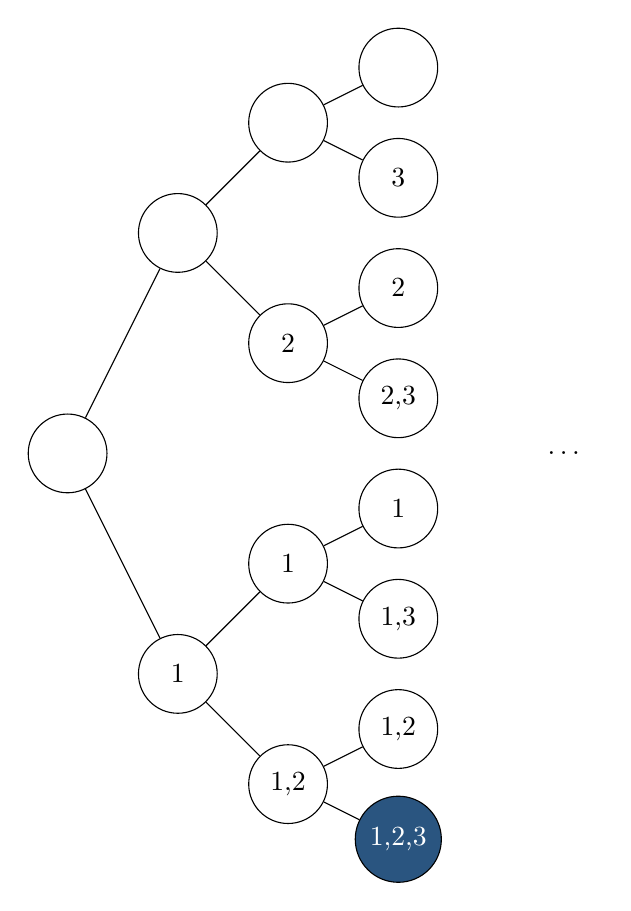
\begin{tikzpicture}[every node/.style={draw,circle, minimum size=1cm}, scale=0.7]
    \node at (0, 7)     (R)         {\(\varnothing\)};

    \node at (2, 11)    (RO)        {\(\varnothing\)};
    \node at (2, 3)     (RA)        {1};

    \node at (4, 13)    (ROO)       {\(\varnothing\)};
    \node at (4, 9)     (ROB)       {2};
    \node at (4, 5)     (RAO)       {1};
    \node at (4, 1)     (RAB)       {1,2};
    
    \node at (6, 14)    (ROOO)      {\(\varnothing\)};
    \node at (6, 12)    (ROOC)      {3};
    \node at (6, 10)    (ROBO)      {2};
    \node at (6, 8)     (ROBC)      {2,3};
    \node at (6, 6)     (RAOO)      {1};
    \node at (6, 4)     (RAOC)      {1,3};
    \node at (6, 2)     (RABO)      {1,2};
    
    % Hervorgehobener Node
    \node[fill={rgb:red,1;green,2;blue,3}] at (6, 0) (RABC) 
        {\textcolor{white}{1,2,3}};
    
    \draw [-] (R) edge (RO) edge (RA);
    \draw [-] (RO) edge (ROO) edge (ROB) (RA) edge (RAB) edge (RAO);
    \draw [-] (ROO) edge (ROOO) edge (ROOC) (ROB) edge (ROBO) edge (ROBC);
    \draw [-] (RAO) edge (RAOO) edge (RAOC) (RAB) edge (RABO) edge (RABC);

    \node[draw=none] at (9, 7) (C) {\(\ldots\)};
\end{tikzpicture}
